\documentclass[11pt,aspectratio=169]{beamer}
\usetheme{Madrid}
\usecolortheme{default}
\usepackage{graphicx}
\usepackage{booktabs}
\usepackage{amsmath}
\usepackage{amsfonts}
\usepackage{hyperref}
\usepackage{natbib}
\usepackage{tikz}
\usepackage{colortbl}
\usetikzlibrary{arrows.meta}
\bibliographystyle{apalike}

\definecolor{taxblue}{RGB}{0,40,104}
\definecolor{policygreen}{RGB}{34,139,34}
\definecolor{peteal}{RGB}{22,163,177}
\setbeamercolor{structure}{fg=taxblue}

\setbeamertemplate{navigation symbols}{}
\setbeamertemplate{footline}[frame number]

\title[Social Security Benefits Taxation]{Simulating Reforms to Taxation of Social Security Benefits}
\subtitle{From Paycheck to Payout: Wealth and Income in Retirement}
\author[Ben Ogorek]{Ben Ogorek\\
Presenting On Behalf of Max Ghenis, Nikhil Woodruff, and Pavel Makarchuk\\
\small{PolicyEngine}}
\institute{118th Annual Conference on Taxation, 2025}
\date{November 7, 2025}

\begin{document}

\begin{frame}
\titlepage
\end{frame}

\begin{frame}{Motivation: A Social Security Policy Reform}
\begin{center}
\large{\textbf{Universal 85\% Inclusion}}
\end{center}

\vspace{0.2cm}
\textbf{Current System (since 1984):}
\begin{itemize}
    \item 0\%, 50\%, or 85\% of benefits taxable
    \item Depends on ``provisional income'' (AGI + half of SS benefits + tax-exempt interest)
    \item Thresholds: \$25k/\$32k (single/joint) and \$34k/\$44k
\end{itemize}

\vspace{0.2cm}
\textbf{Proposed Reform:}
\begin{itemize}
    \item \textbf{85\% of all benefits taxable}, regardless of income
    \item Eliminates threshold system entirely
\end{itemize}
\end{frame}

\begin{frame}[fragile]{How the Reform is Implemented in PolicyEngine}
\begin{center}
\textbf{Python Implementation in PolicyEngine}
\end{center}

\vspace{0.2cm}
\tiny
\begin{verbatim}
def tax_85_percent_ss():
    """Tax 85% of Social Security benefits for all recipients."""
    return {
        # Set combined income fraction to 1.0 (instead of 0.5)
        "gov.irs.social_security.taxability.combined_income_ss_fraction": {
            "2026-01-01.2100-12-31": 1.0
        },
        # Set all base thresholds to 0
        "gov.irs.social_security.taxability.threshold.base.main.JOINT": {
            "2026-01-01.2100-12-31": 0
        },
        "gov.irs.social_security.taxability.threshold.base.main.SINGLE": {
            "2026-01-01.2100-12-31": 0
        },
        # ... (all other filing statuses)

        # Set all adjusted base thresholds to 0
        "gov.irs.social_security.taxability.threshold.adjusted_base.main.JOINT": {
            "2026-01-01.2100-12-31": 0
        },
        "gov.irs.social_security.taxability.threshold.adjusted_base.main.SINGLE": {
            "2026-01-01.2100-12-31": 0
        },
        # ... (all other filing statuses)
    }
\end{verbatim}

\end{frame}

\begin{frame}{Explore the Code Yourself}
\begin{center}
\Large{\textbf{PolicyEngine is Open Source}}
\end{center}

\vspace{0.3cm}

\begin{center}
\textcolor{peteal}{\textbf{\large \url{https://github.com/PolicyEngine/policyengine-us}}}
\end{center}

\vspace{0.4cm}

\begin{columns}
\begin{column}{0.32\textwidth}
\begin{center}
\textcolor{policygreen}{\Large \textbf{/}}

\vspace{0.2cm}
\textbf{policyengine\_us/\\parameters/}

\vspace{0.2cm}
\small
All tax code parameters in YAML

Tax rates, thresholds, credits, deductions, elasticities
\end{center}
\end{column}

\begin{column}{0.32\textwidth}
\begin{center}
\textcolor{taxblue}{\Large \textbf{/}}

\vspace{0.2cm}
\textbf{policyengine\_us/\\variables/}

\vspace{0.2cm}
\small
Income, tax, benefit calculations

The computational logic that implements the tax code
\end{center}
\end{column}

\begin{column}{0.32\textwidth}
\begin{center}
\textcolor{peteal}{\Large \textbf{/}}

\vspace{0.2cm}
\textbf{policyengine\_us/\\reforms/}

\vspace{0.2cm}
\small
Policy reform definitions

Pre-built reforms you can use or customize
\end{center}
\end{column}
\end{columns}

\vspace{0.4cm}

\end{frame}

\begin{frame}{Simulated Reform Revenue Impacts of Universal 85\% Inclusion}
\vspace{-0.1cm}
\begin{center}
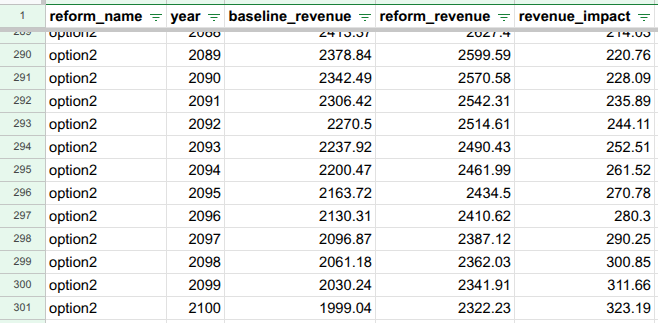
\includegraphics[width=0.48\textwidth]{figures/Option2_2100.png}
\end{center}

\vspace{0.1cm}
  This particular (very much in beta) simulation run:
\small
\begin{itemize}
    \item Incorporates \textbf{labor supply elasticities} (dynamic behavioral response)
    \item Reflects \textbf{demographic changes} over 75-year horizon
    \item Could be extended to do distributional analysis with income, age, etc.
\end{itemize}
  \textbf{The Rest of the Presentation is about Showing How We Got Here}
\end{frame}

\section{Dynamic Behavioral Modeling}

\begin{frame}{Behavioral Responses in PolicyEngine: Labor Supply Elasticities}

\vspace{0.2cm}
\textbf{Two Key Parameters in PolicyEngine:}

\vspace{0.15cm}
\textcolor{policygreen}{\textbf{Income Elasticity}}
\begin{itemize}
\item \footnotesize\texttt{gov.simulation.labor\_supply\_responses.elasticities.income}
\item Default: 0 (no response)
\item CBO estimate: -0.04
\end{itemize}

\vspace{0.15cm}
\textcolor{taxblue}{\textbf{Substitution Elasticity}}
\begin{itemize}
\item \footnotesize\texttt{gov.simulation.labor\_supply\_responses.elasticities.substitution}
\item Default: 0 (no response)
\item CBO estimate: 0.27
\end{itemize}


\end{frame}

\begin{frame}[fragile]{How Elasticities Flow Through the Engine}
\begin{center}
\textbf{The Complete Calculation Chain}
\end{center}

\vspace{0.2cm}
\scriptsize

\textbf{1. Elasticity parameters} (YAML files: \texttt{base.yaml}, \texttt{by\_position\_and\_decile.yaml})

$\downarrow$

\textbf{2. Read and apply adjustments} (\texttt{income\_elasticity}, \texttt{substitution\_elasticity} variables)

$\downarrow$

\textbf{3. Multiply by earnings/wage changes} (\texttt{income\_elasticity\_lsr}, \texttt{substitution\_elasticity\_lsr})

$\downarrow$

\textbf{4. Sum the two effects} (\texttt{labor\_supply\_behavioral\_response})

$\downarrow$

\textbf{5. Allocate by employment share} (\texttt{employment\_income\_behavioral\_response})

$\downarrow$

\textbf{6. Add to base income} (\texttt{employment\_income})

\vspace{0.3cm}

\begin{verbatim}
# employment_income.py
class employment_income(Variable):
    adds = [
        "employment_income_before_lsr",
        "employment_income_behavioral_response",  # <-- Contains the LSR
    ]
\end{verbatim}

\end{frame}

\begin{frame}{Extension: Age Heterogeneity of Labor Supply Elasticity}
\begin{center}
\textbf{Empirical finding:} Workers 65+ are significantly more responsive\\
to economic incentives

\vspace{0.3cm}

\textbf{Evidence from Literature:}

\vspace{0.2cm}
\small
\begin{tabular}{lcc}
\toprule
\textbf{Study} & \textbf{Age} & \textbf{$65+/<65$ Ratio} \\
\midrule
French (2005) & 60 vs 40 & 3.0–3.25× \\
Blau \& Shvydko (2011) & 62–69 & 2.0–3.0× \\
Gustman \& Steinmeier (2009) & 65–69 & 2.0–2.5× \\
\bottomrule
\end{tabular}

\vspace{0.3cm}
\normalsize
\textbf{PolicyEngine Default (But Tunable) Implementation:}
\begin{equation*}
\varepsilon_{\text{age} \geq 65} = 2.0 \times \varepsilon_{\text{age} < 65}
\end{equation*}
\end{center}

\end{frame}

\begin{frame}[fragile]{Age Multiplier Implementation}
\begin{center}
\textbf{How PolicyEngine Applies the Age-Based Elasticity Multiplier in Code}
\end{center}

\vspace{0.2cm}
\tiny

\textbf{Income Elasticity (income\_elasticity.py):}
\begin{verbatim}
age = person("age", period.this_year)
age_multiplier = where(
    age >= p.age_threshold,                 # <-- PARAMETER from YAML (65)
    p.age_multiplier_over_threshold,        # <-- PARAMETER from YAML (2.0)
    1.0,                                    # No multiplier for under threshold
)

return base_elasticity * age_multiplier
\end{verbatim}

\vspace{0.2cm}

\textbf{Substitution Elasticity (substitution\_elasticity.py):}
\begin{verbatim}
age = person("age", period.this_year)
age_multiplier = where(
    age >= p.age_threshold,                 # <-- PARAMETER from YAML (65)
    p.age_multiplier_over_threshold,        # <-- PARAMETER from YAML (2.0)
    1.0,                                    # No multiplier for under threshold
)

return base_elasticity * age_multiplier
\end{verbatim}

\vspace{0.2cm}
\scriptsize
\textbf{Result:} Same simple logic for both elasticities. Workers 65+ get 2× multiplier; workers under 65 get 1× (no change).

\end{frame}

\begin{frame}[fragile]{A PolicyEngine Test Case That Sets Elasticity Parameters}
\vspace{0.2cm}
\tiny
\begin{verbatim}
# PolicyEngine US Parameter Settings (YAML)

# Income elasticity parameters
gov.simulation.labor_supply_responses.elasticities.income:
  all: -0.04                           # CBO central estimate
  age_multiplier_over_threshold: 2.0   # 65+ workers 2x more responsive
  age_threshold: 65                    # Age cutoff for multiplier

# Substitution elasticity parameters
gov.simulation.labor_supply_responses.elasticities.substitution:
  all: 0.27                            # CBO central estimate
  age_multiplier_over_threshold: 2.0   # 65+ workers 2x more responsive
  age_threshold: 65                    # Age cutoff for multiplier

# Result:
#   - Workers under 65: income_elasticity = -0.04,  substitution_elasticity = 0.27
#   - Workers 65+:      income_elasticity = -0.08,  substitution_elasticity = 0.54
\end{verbatim}

\vspace{0.1cm}
\scriptsize
\textbf{Default:} All elasticities = 0 (static analysis). Must explicitly enable for dynamic modeling.

\vspace{0.1cm}
\textbf{References embedded in parameters:} French (2005), CBO Working Papers 2012-12 \& 2012-13
\end{frame}

\section{Data and Methodology}
\begin{frame}{Source Data}
\begin{columns}
\begin{column}{0.5\textwidth}
    \textbf{Survey Dataset}
    \begin{itemize}
        \item CPS ASEC (March Supplement)
        \item \textasciitilde180k individuals
        \item Demographics + basic income
    \end{itemize}
\end{column}
\begin{column}{0.5\textwidth}
    \textbf{Administrative Dataset}
    \begin{itemize}
        \item IRS Statistics of Income
        \item \textasciitilde207k tax filers, 120k with demographics
        \item Actual Tax filings 
    \end{itemize}
\end{column}
\end{columns}

\vspace{0.5cm}
\begin{block}{Data Fusion Strategy}
Use Quantile Regression Forests to impute conditional income distributions from IRS PUF onto CPS households
\end{block}
\end{frame}

\begin{frame}{Data Fusion: Quantile Regression Forests}
\textbf{Problem:} Simple mean imputation loses distributional information

\vspace{0.3cm}
\textbf{Solution:} Quantile Regression Forests (QRF)
\begin{enumerate}
    \item Train QRF on matched administrative-survey data
    \item Generate full conditional distributions for each household
    \item Preserve complex demographic-income relationships
\end{enumerate}

\vspace{0.3cm}
\begin{equation*}
\hat{F}_{Y|X}(y|x) = \sum_{i=1}^{n} w_i(x) \cdot \mathbf{1}\{Y_i \leq y\}
\end{equation*}

Where $w_i(x)$ are forest-derived weights based on similarity
\end{frame}

\begin{frame}{Why We Want to Impute Income (Sometimes)}
\begin{columns}
\begin{column}{0.48\textwidth}
\textbf{CPS Issue: Rank Proximity Swapping (RPS)}

\vspace{0.3cm}
\textbf{Post-2011:} Income values swapped among similar-ranked households

\vspace{0.2cm}
$$(\mathbf{I}_j^{\text{CPS}}, \mathbf{D}_j) = (I_{\pi(j)}^{\text{true}}, \mathbf{D}_j^{\text{true}})$$

\vspace{0.2cm}
\textbf{Impact:} Destroys joint distribution

$$\text{Cov}(I^{\text{CPS}}, X^{\text{CPS}}) \neq \text{Cov}(I^{\text{true}}, X^{\text{true}})$$

\end{column}

\begin{column}{0.48\textwidth}
\textbf{Why This Matters for Tax Microsimulation}

\begin{itemize}
    \item 65-year-old household gets 35-year-old's income
    \item Tax function is nonlinear: $T = \mathcal{T}(\mathbf{I}, \mathbf{D})$
    \item Wrong demographics → biased tax calculations
    \item Upper tail especially affected
\end{itemize}

\end{column}
\end{columns}
\end{frame}

\begin{frame}{Dual-Source Data Fusion Pipeline}
\begin{center}
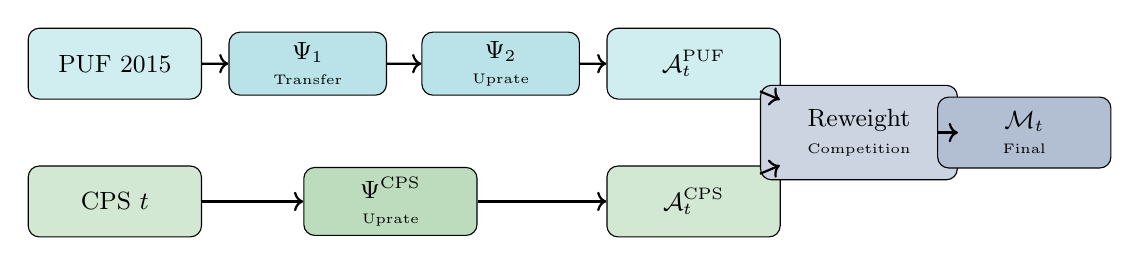
\begin{tikzpicture}[scale=0.7]
    % PUF track
    \node[draw, fill=peteal!20, rounded corners, minimum width=2.2cm, minimum height=0.9cm, align=center]
        (puf0) at (0,2) {\small PUF 2015};
    \node[draw, fill=peteal!30, rounded corners, minimum width=2cm, minimum height=0.8cm, align=center]
        (psi1) at (3.5,2) {\small $\Psi_1$\\[-3pt]\tiny Transfer};
    \node[draw, fill=peteal!30, rounded corners, minimum width=2cm, minimum height=0.8cm, align=center]
        (psi2) at (7,2) {\small $\Psi_2$\\[-3pt]\tiny Uprate};
    \node[draw, fill=peteal!20, rounded corners, minimum width=2.2cm, minimum height=0.9cm, align=center]
        (puft) at (10.5,2) {\small $\mathcal{A}_t^{\text{PUF}}$};

    \draw[->, thick] (puf0) -- (psi1);
    \draw[->, thick] (psi1) -- (psi2);
    \draw[->, thick] (psi2) -- (puft);

    % CPS track
    \node[draw, fill=policygreen!20, rounded corners, minimum width=2.2cm, minimum height=0.9cm, align=center]
        (cps0) at (0,-0.5) {\small CPS $t$};
    \node[draw, fill=policygreen!30, rounded corners, minimum width=2.2cm, minimum height=0.8cm, align=center]
        (psicps) at (5,-0.5) {\small $\Psi^{\text{CPS}}$\\[-3pt]\tiny Uprate};
    \node[draw, fill=policygreen!20, rounded corners, minimum width=2.2cm, minimum height=0.9cm, align=center]
        (cpst) at (10.5,-0.5) {\small $\mathcal{A}_t^{\text{CPS}}$};

    \draw[->, thick] (cps0) -- (psicps);
    \draw[->, thick] (psicps) -- (cpst);

    % Reweighting stage
    \node[draw, fill=taxblue!20, rounded corners, minimum width=2.5cm, minimum height=1.2cm, align=center]
        (reweight) at (13.5,0.75) {\small Reweight\\[-2pt]\tiny Competition};
    \node[draw, fill=taxblue!30, rounded corners, minimum width=2.2cm, minimum height=0.9cm, align=center]
        (final) at (16.5,0.75) {\small $\mathcal{M}_t$\\[-3pt]\tiny Final};

    \draw[<-, thick] (puft) -- (reweight);
    \draw[<-, thick] (cpst) -- (reweight);
    \draw[<-, thick] (reweight) -- (final);
\end{tikzpicture}
\end{center}

\vspace{0.1cm}

\begin{columns}
\begin{column}{0.48\textwidth}
\textbf{PUF Track:} Admin data foundation
\begin{itemize}
    \item $\Psi_1$: Transfer CPS patterns for missing variables \textit{while preserving PUF income}
    \item $\Psi_2$: Uprate 2015 → $t$ via uprating factors 
\end{itemize}

\textbf{CPS Track:} $\Psi^{\text{CPS}}$ Uprate 2023 → $t$ via uprating factors
\end{column}

\begin{column}{0.48\textwidth}
\textbf{Reweighting Competition:}
\begin{itemize}
    \item PUF dominates upper tail (no RPS contamination)
    \item CPS contributes rich demographics
    \item Optimal weights via constrained optimization
\end{itemize}
$$\mathcal{M}_t = \text{Reweight}(\mathcal{A}_t^{\text{PUF}} \cup \mathcal{A}_t^{\text{CPS}})$$
\end{column}
\end{columns}
\end{frame}


\begin{frame}{Dual-Source Competitive Reweighting}

\begin{center}
\textbf{Final Dataset Construction:} $\mathcal{M}_t = \text{Reweight}(\mathcal{A}_t^{\text{PUF}} \cup \mathcal{A}_t^{\text{CPS}})$
\end{center}

\vspace{0.3cm}

\begin{columns}
\begin{column}{0.55\textwidth}
  \textbf{Use PyTorch to Approximately Solve:}

\vspace{0.2cm}
$$\mathbf{t} = \mathbf{X}\mathbf{w}$$

\vspace{0.2cm}
\begin{itemize}
    \item $\mathbf{t}$: Calibration targets
    \item $\mathbf{X}$: Household characteristics matrix
    \item $\mathbf{w}$: Household weights
\end{itemize}

\vspace{0.3cm}
\textbf{Calibration Target Categories:}
\begin{itemize}
    \item IRS SOI statistics
    \item Benefit program participation rates
    \item Demographic distributions
\end{itemize}

\end{column}

\begin{column}{0.4\textwidth}
\textbf{Competition Outcome:}

\vspace{0.3cm}

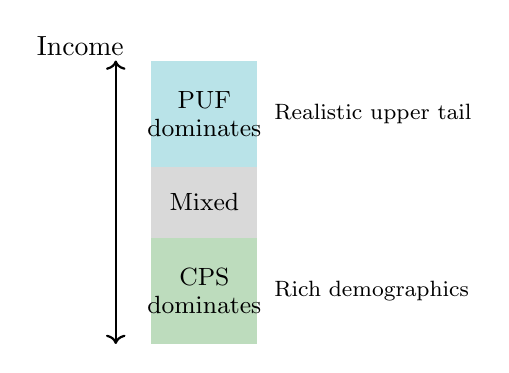
\begin{tikzpicture}[scale=0.9]
    \draw[<->, thick] (0,0) -- (0,4);
    \node at (-0.5,4.2) {Income};

    \fill[policygreen!30] (0.5,0) rectangle (2,1.5);
    \node[align=center] at (1.25,0.75) {\small CPS\\[-2pt]\small dominates};

    \fill[gray!30] (0.5,1.5) rectangle (2,2.5);
    \node[align=center] at (1.25,2) {\small Mixed};

    \fill[peteal!30] (0.5,2.5) rectangle (2,4);
    \node[align=center] at (1.25,3.25) {\small PUF\\[-2pt]\small dominates};

    \node[right, align=left] at (2.1,0.75) {\footnotesize Rich demographics};
    \node[right, align=left] at (2.1,3.25) {\footnotesize Realistic upper tail};
\end{tikzpicture}

\end{column}
\end{columns}

\vspace{0.3cm}

\begin{block}{Key Advantage}
Exploits complementary strengths: PUF's unperturbed admin data for high incomes + CPS's comprehensive demographics for broader population
\end{block}

\end{frame}


\section{75-Year Projection Methodology}

\begin{frame}{Projecting to 2100 requires modeling both economic and demographic evolution}

\vspace{0.3cm}

\begin{columns}
\begin{column}{0.48\textwidth}
\textbf{Economic Evolution}
\begin{itemize}
    \item Wage growth
    \item Inflation rates 
    \item Population growth (for uprating of weights) 
\end{itemize}

\vspace{0.2cm}
\textcolor{policygreen}{\textbf{Source: CBO or SSA Trustees projections}}
\end{column}

\begin{column}{0.48\textwidth}
\textbf{Demographic Transformation}
\begin{itemize}
    \item Baby boom aging
    \item Declining birth rates
    \item Increasing longevity
\end{itemize}

\vspace{0.2cm}
\textcolor{peteal}{\textbf{Source: SSA Trustees Report}}
\end{column}
\end{columns}

\vspace{0.3cm}

\begin{center}
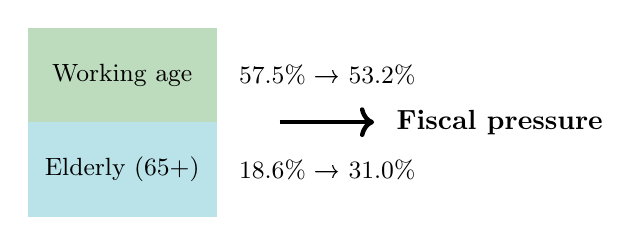
\begin{tikzpicture}[scale=0.8]
    % Working age shrinking
    \fill[policygreen!30] (0,0) rectangle (3,1.5);
    \node at (1.5,0.75) {\small Working age};
    \node[right] at (3.2,0.75) {\small 57.5\% → 53.2\%};

    % Elderly expanding
    \fill[peteal!30] (0,-1.5) rectangle (3,-0);
    \node at (1.5,-0.75) {\small Elderly (65+)};
    \node[right] at (3.2,-0.75) {\small 18.6\% → 31.0\%};

    \draw[->, ultra thick] (4,0) -- (5.5,0);
    \node[right] at (5.7,0) {\textbf{Fiscal pressure}};
\end{tikzpicture}
\end{center}

\vspace{0.1cm}
\textbf{Traditional tradeoff:} Sacrifice either economic sophistication OR demographic realism

\textbf{Our approach:} Preserve both through two-stage methodology
\end{frame}

\begin{frame}{After the Economic Evolution Based on Factors: Reweighting (Again!)}

  We'll use a more traditional calibration that minimizes distance to the ``original weights'' (our reweighted weights from before) while satisfying the following auxiliary constraints: 

\small
\begin{itemize}
    \item \textbf{Age-specific targets}: Single-year ages 0-85+ through 2100
    \item \textbf{SS benefit totals}: Match SSA Trustees Report Table VI.G9
\end{itemize}

  \textbf{GREG} is the \textbf{Generalized Regression Estimator} calibrator.

\begin{itemize}
   \item Raking could have been used, if it wasn't for the continuous SS Benefit variable.
   \item Now we want our calibrated weights to not move too far, so we use a traditional calibration procedure that
   \item minimizes a distance from the new weights to the original weights subject to the auxiliary constraints.
\end{itemize}
\end{frame}

\begin{frame}
\begin{center}
\Large{\textbf{Thank You!}}

\vspace{0.5cm}
Ben.Ogorek@PolicyEngine.org \\
Max@PolicyEngine.org \\
Nikhil@PolicyEngine.org \\
Pavel@PolicyEngine.org \\
\vspace{0.5cm}
\textbf{Resources:}\\
\url{https://policyengine.org}
\end{center}
\end{frame}

\end{document}
